% 230V relæ modultest

Efter godkendelse af relæet ved Torben Lund Jensen er relæets funktion testet. 
Laboratoriets spændingsforsyning er indstillet til 4 V og 100mA som er det relæet modtager fra tilslutningsprintet.
Apparatstikket tilsluttes en aktiv 230V stikkontakt, bananbøsningerne tilsluttes laboratorie spændingsforsyningen.
Et multimeter indstilles til vekselstrøm om målepindene indsættes i stikkontakten på relækassen. 

Figur \ref{lab:Relay_moduletest} viser outputtet når relæet er klikket. Som det ses er stikkontakten tændt med en spænding på 232,2Vac. Når relæet afbrydes slukkes stikkontakten som forventet.

\begin{figure}[htb]
\centering
{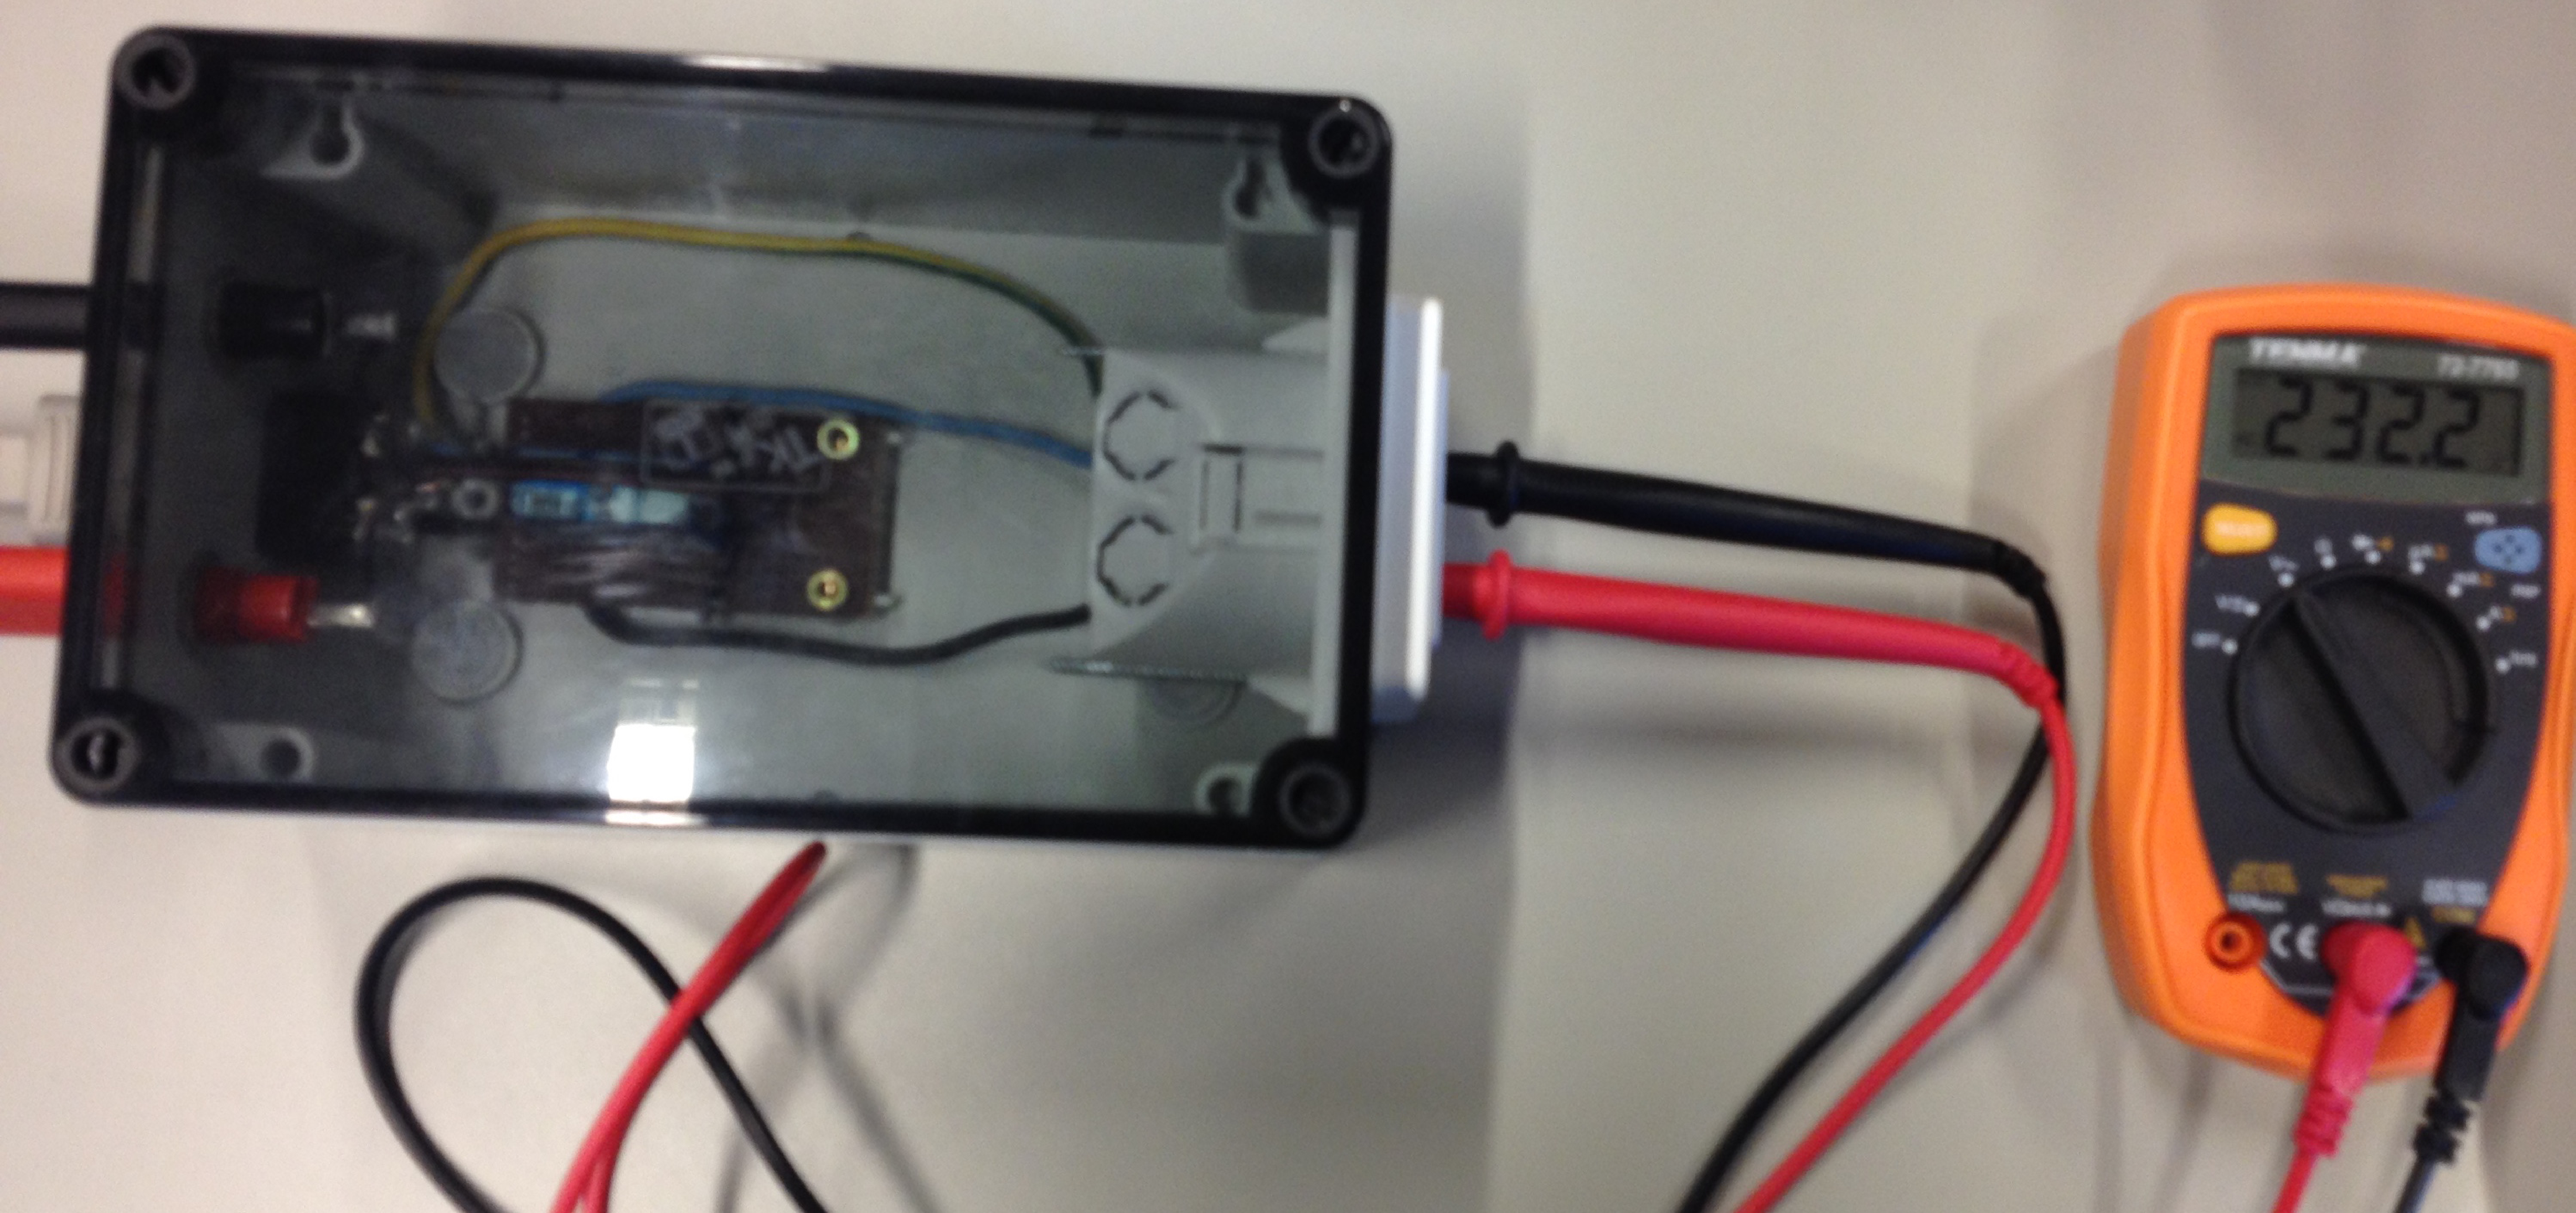
\includegraphics[width=0.80\textwidth]{filer/modultest/billeder/230Vrelay_modultest}}
\caption{Aktivt relæ med 232 Vac på udgangen }
\label{lab:Relay_moduletest}
\end{figure}


